\documentclass[11pt]{article}
\usepackage[margin=1in]{geometry}
\usepackage{setspace}
\usepackage{amsmath,amssymb}
\usepackage{graphicx}
\usepackage{booktabs}
\usepackage{array}
\usepackage{float}
\usepackage{caption}
\usepackage{algorithm}
\usepackage{algpseudocode}
\usepackage{etoolbox}
\usepackage[hidelinks]{hyperref}

\setstretch{1.15}
\AtBeginEnvironment{algorithmic}{\setstretch{1.0}}
\AtBeginEnvironment{tabular}{\setstretch{1.0}}
\captionsetup{font=small,skip=4pt}
\setlength{\textfloatsep}{8pt}
\setlength{\intextsep}{6pt}

% Advantages and limitations of one approach.
\newcommand{\proscons}[3]{%
\par\smallskip\noindent{\footnotesize
\begin{tabular}{|p{0.455\linewidth}|p{0.455\linewidth}|}
\hline
\textbf{Advantages of #3} & \textbf{Limitations of #3} \\
\hline
#1 & #2 \\
\hline
\end{tabular}}\par\smallskip}

\title{\textbf{Observability-Aware Trust-Based Grayhole Detection for Underwater Acoustic Networks}\\[4pt]
\large Final Report}
\date{November 2, 2026}

\begin{document}
\maketitle

\section*{Team Members}
\noindent 1. 241CS110, Appaji Nagaraja Dheeraj, appajidheeraj.241cs110@nitk.edu.in, 9481660290 \\
\noindent 2. 241CS111, Aryan Bokolia, aryanbokolia.241cs111@nitk.edu.in, 7982212773 \\
\noindent 3. 241CS117, Karthikeya Gupta, karthikeyagupta.241cs117@nitk.edu.in, 6303223736

\section*{Abstract}
\noindent
Underwater acoustic sensor networks send data from seabed sensors to a surface sink over several relay hops~\cite{akyildiz2005}.
A captured relay can drop a part of the packets that it must forward.
This is a grayhole attack, and encryption does not stop it, because the relay keeps its keys~\cite{karlof2003,domingo2011}.
The usual defence is a watchdog, in which a node listens for its next hop to forward each packet and accuses the next hop when too many forwards are missing~\cite{marti2000}.
Under water, a forward is also missing when the half-duplex monitor transmits at that time, when the packet collides at the relay, or when a long link loses it.
These losses increase with traffic, so a fixed threshold accuses honest relays or misses grayholes.
We built a detector in UnetStack~7~\cite{chitre2014} that counts a watch window only when the monitor was able to observe the forward.
It compares the forwards heard with the forwards that an honest relay must show on each link, from the link distance and the normal loss of links of a similar length.
The sink receives the evidence in reports over the acoustic channel, ranks the relays and confirms suspects over two rounds.
We compared the detector with a fixed-threshold watchdog and a channel-aware (CAD-style) detector on ten test networks.
In the live network, it catches 95\% of the grayholes and accuses 0.3 honest relays per run, and the fixed watchdog accuses 7.2.
The delivery ratio is the percentage of the data packets from honest sensors that arrive at the sink.
When the sink blacklists the suspects, the delivery ratio with our detector is 45.7\%, and with the fixed watchdog it is 23.2\%.
This is an absolute increase of 22.6\% in the delivery ratio.

%==========================================================
\clearpage
\section{Introduction}\label{sec:intro}

\subsection{Background}\label{sec:background}
\noindent
Underwater acoustic sensor networks (UASNs) collect data for ocean sampling, pollution monitoring, offshore exploration and tactical surveillance~\cite{akyildiz2005,brc2021}.
Radio waves lose their energy within a few metres of sea water, so underwater nodes use acoustic modems.
Sound moves at about 1500~m/s.
Thus the propagation delay is five orders of magnitude longer than on a terrestrial radio link~\cite{akyildiz2005}.
The usable bandwidth is only a few kilohertz, and it decreases as the link distance increases.
Multipath and fading cause a high bit error rate, and the nodes use batteries that are difficult to replace~\cite{akyildiz2005}.

A sensor on the seabed seldom reaches the sink directly.
It sends its packets to a neighbour, and the neighbour sends them on, until they arrive at the sink, which is usually a surface buoy.
The network layer selects these relays, so each node depends on its relays to forward its packets~\cite{brc2021}.
This dependence is a security problem.
Nodes stay at sea without supervision for months, so an attacker can capture a node and change its software~\cite{domingo2011,jiang2019}.
The captured node keeps its keys and stays in the routes, so encryption does not stop it.

Karlof and Wagner call this attack selective forwarding~\cite{karlof2003}.
A node that drops all packets is a blackhole.
The traffic through it stops, so it is easy to find.
A node that drops only a part of the packets, for example 30\%, is a grayhole.
Honest acoustic links also lose frames, so the drops of a grayhole look like normal link loss~\cite{akyildiz2005,domingo2011}.
UnetStack is a network stack and simulator for UASNs, and its agents can also run on real modems~\cite{chitre2014}.
Dr.~B.~R.~Chandavarkar and N.~Suresh used UnetStack3 to show a selective forwarding attack and its detection on a four-node network~\cite{brc2021}.
We use UnetStack~7 for this project.

Domingo lists selective forwarding among the main attacks on underwater networks, together with jamming, wormhole, sinkhole, HELLO flood and Sybil attacks~\cite{domingo2011}.
A grayhole is more difficult to find than a blackhole, because it stays in the routes and drops only a part of the traffic~\cite{karlof2003}.
The packets that it drops are lost.
Underwater sensors have little memory and energy, and the long delays make retransmission expensive~\cite{akyildiz2005}.
Thus a grayhole on a busy relay decreases the data that arrives at the sink for every sensor behind it.
In our test networks, one grayhole on the busiest relay decreases the delivery ratio by 8.4\%, and three grayholes decrease it by 17.0\% (Section~\ref{sec:res-attack}).

\subsection{Challenges and issues}\label{sec:challenges}
\noindent
A watchdog uses silence as evidence~\cite{marti2000}.
Under water, a silence has many causes, and only one of them is a drop by the relay.
First, acoustic modems are usually half-duplex, so the monitor cannot receive the forward while it transmits.
Second, a relay that transmits while the packet arrives does not receive the packet and has nothing to forward.
Third, the packet can collide at the relay with a frame from a third node that the monitor cannot hear.
Marti et al.\ list such receiver collisions and ambiguous collisions as weak points of the watchdog~\cite{marti2000}.
Fourth, the link from the relay back to the monitor can lose the forward, and a long link loses more frames than a short link~\cite{akyildiz2005}.

These innocent misses increase with traffic, because more traffic causes more collisions and more time in transmission.
Thus, even with no attacker, a monitor misses more honest forwards when the load is high.
A low fixed threshold then accuses honest relays at high load, and a high threshold misses grayholes at low load.
The loss also changes from link to link, so one threshold for all links is incorrect for most links~\cite{shila2010}.

False accusations have a cost.
Traffic that goes around an accused relay uses longer paths, with more hops and more collisions.
If the accused relay is the only path for some nodes, its removal disconnects them.
Probe and acknowledgement packets use energy and channel time, which a UASN cannot easily give~\cite{akyildiz2005,brc2021}.
Two or three grayholes in one area increase the loss that a detector thinks is normal, and this can hide all of them.
Finally, the evidence must go to the sink over the same lossy channel.

\subsection{Existing approaches and their issues}\label{sec:existing}
\noindent
The watchdog of Marti et al.\ counts each missing forward against the next hop and uses one fixed threshold~\cite{marti2000}.
Hai and Huh let neighbour nodes watch a relay and use two-hop neighbour lists to find a forward to a wrong node~\cite{hai2008}.
Dr.~B.~R.~Chandavarkar and N.~Suresh adapted this method for UnetStack3, with the destination as the only monitor~\cite{brc2021}.
The destination keeps one counter for missing packets and one for packets with a wrong destination, and raises an alarm when a counter goes above a fixed threshold.
These counter methods count every silence as a drop.
Channel-aware detection (CAD) by Shila et al.\ estimates the normal loss from channel errors and collisions and sets its thresholds from that loss~\cite{shila2010}.
CAD is for terrestrial mesh networks and needs probe packets and signed link-layer acknowledgements.
It also gets collisions from an average busy ratio, not from a check of each observation.
Underwater trust models such as ARTMM~\cite{han2015}, TAFLRLR~\cite{han2023} and ATEM~\cite{liu2024} combine link, data and energy evidence, and ATEM stops a trust cycle when the link is unstable.
These models judge a relay from counts of good and bad interactions.
None of them checks, for each watched packet, whether the monitor was able to hear the forward.

\subsection{Problem statement}\label{sec:problem}
\noindent
In a static multi-hop UASN, some relays drop a part of the packets that they must forward.
We must design a network-layer detector that uses only what each node observes, plus the known node positions and channel loss curve.
It must find the grayholes and accuse few honest relays, also at high traffic and with more than one grayhole.
Its evidence must go to the sink over the acoustic channel, and the sink must then keep traffic away from the suspects.

\subsection{Objectives}\label{sec:objectives}
\begin{enumerate}\setlength{\itemsep}{0pt}
  \item Build in UnetStack a watchdog that counts a window only when the monitor was able to observe the forward, and that compares the forwards heard with the forwards expected on each link.
  \item Compare it with a fixed-threshold watchdog and a CAD-style detector on the same recorded traffic, with thresholds tuned on networks that we do not use for the test.
  \item Measure grayholes caught, honest relays accused and delivery ratio in a live simulated network with reports, route changes and blacklisting.
\end{enumerate}

\subsection{Organization of the report}\label{sec:organization}
\noindent
Section~\ref{sec:lit} reviews the existing approaches in the order of publication and compares them in Section~\ref{sec:lit-compare}.
Section~\ref{sec:prop} gives our detector, its algorithm and the reason for each design choice.
Section~\ref{sec:impl} describes the implementation in UnetStack, with the class diagram and the pseudocode of the main functions.
Section~\ref{sec:results} gives the simulation parameters, the scenarios, the metrics and the results, and compares our detector with the baselines and the reviewed approaches.
Section~\ref{sec:conclusion} gives the conclusions and the future work.

%==========================================================
\section{Literature review}\label{sec:lit}
\noindent
We review seven approaches in the order of publication.
For each approach, we give our own algorithm or diagram and its advantages and limitations.

\subsection{Watchdog and pathrater (2000)}\label{sec:lit-watchdog}
\noindent
Marti et al.\ proposed the watchdog and the pathrater for mobile ad hoc networks~\cite{marti2000}.
A sender keeps a copy of each packet and listens for its next hop to send it again.
If the copy stays longer than a timeout, the sender increases a failure count for the next hop.
When the count crosses a threshold, the sender reports the next hop to the source, and the pathrater selects a path without it (Algorithm~\ref{alg:watchdog}).

\begin{figure}[H]
\centering
\begin{minipage}[t]{0.47\linewidth}
\captionof{algorithm}{Watchdog at a sender~\cite{marti2000}}\label{alg:watchdog}
\footnotesize
\begin{algorithmic}[1]
\State Send $P$ to next hop $B$; keep a copy of $P$
\If{$B$ does not send $P$ again before the timeout}
  \State $\mathit{fail}_B \gets \mathit{fail}_B + 1$ \Comment{any silence}
\EndIf
\If{$\mathit{fail}_B > \theta$}
  \State Report $B$ to the source; pathrater avoids $B$
\EndIf
\end{algorithmic}
\end{minipage}\hfill
\begin{minipage}[t]{0.49\linewidth}
\captionof{algorithm}{Two-hop monitoring~\cite{hai2008,brc2021}}\label{alg:twohop}
\footnotesize
\begin{algorithmic}[1]
\State Overhear $P$ from $A$ to $B$, both one-hop neighbours
\State Keep $P$ with a timer $\tau$
\If{$B$ forwards $P$ to a node not in the two-hop list of $A$}
  \State Send an alert with factor $\beta$ to the source
\ElsIf{$\tau$ expires before the forward}
  \State Send an alert with factor $\alpha$ to the source
\EndIf
\end{algorithmic}
\end{minipage}
\end{figure}

\proscons{No extra packets for detection. Each node watches its own next hop, so detection is distributed. Simple to implement.}
{The authors list ambiguous and receiver collisions, collusion and partial dropping as weak points. Every silence counts, with one fixed threshold for all links.}
{the watchdog}

\subsection{Two-hop neighbour monitoring (2008)}\label{sec:lit-twohop}
\noindent
Hai and Huh proposed a distributed method for wireless sensor networks, in which any neighbour of a relay can be a monitor~\cite{hai2008}.
Dr.~B.~R.~Chandavarkar and N.~Suresh used it as the base of their UnetStack3 detector, and their paper gives its algorithm~\cite{brc2021}, which Algorithm~\ref{alg:twohop} follows.
A monitor sends an alert with factor $\beta$ when the relay forwards off the path, and with factor $\alpha$ when its timer expires.

\proscons{More than one monitor can watch a relay. It also finds a forward to a wrong node. Distributed, with no central node.}
{Alert packets use energy and channel time. An expired timer counts as an alert, whatever caused the silence. There is no model of normal link loss.}
{two-hop monitoring}

\subsection{Channel-aware detection (2010)}\label{sec:lit-cad}
\noindent
Shila, Cheng and Anjali designed channel-aware detection (CAD) for grayholes in wireless mesh networks~\cite{shila2010}.
Each node counts the packets from its upstream node, keeps the signed link-layer acknowledgements of its downstream node and listens for the forward.
The normal loss of a link is $p_r = p_e + p_o - p_e p_o$, where $p_e$ is the channel loss and $p_o$ is the collision probability from the channel busy ratio.
The thresholds minimise the sum of the false alarm and missed detection probabilities and follow $p_r$.
PROBE and PROBE-ACK packets confirm the path, and the authors evaluate CAD in NS2 (Figure~\ref{fig:cad}).

\begin{figure}[!htb]
\centering
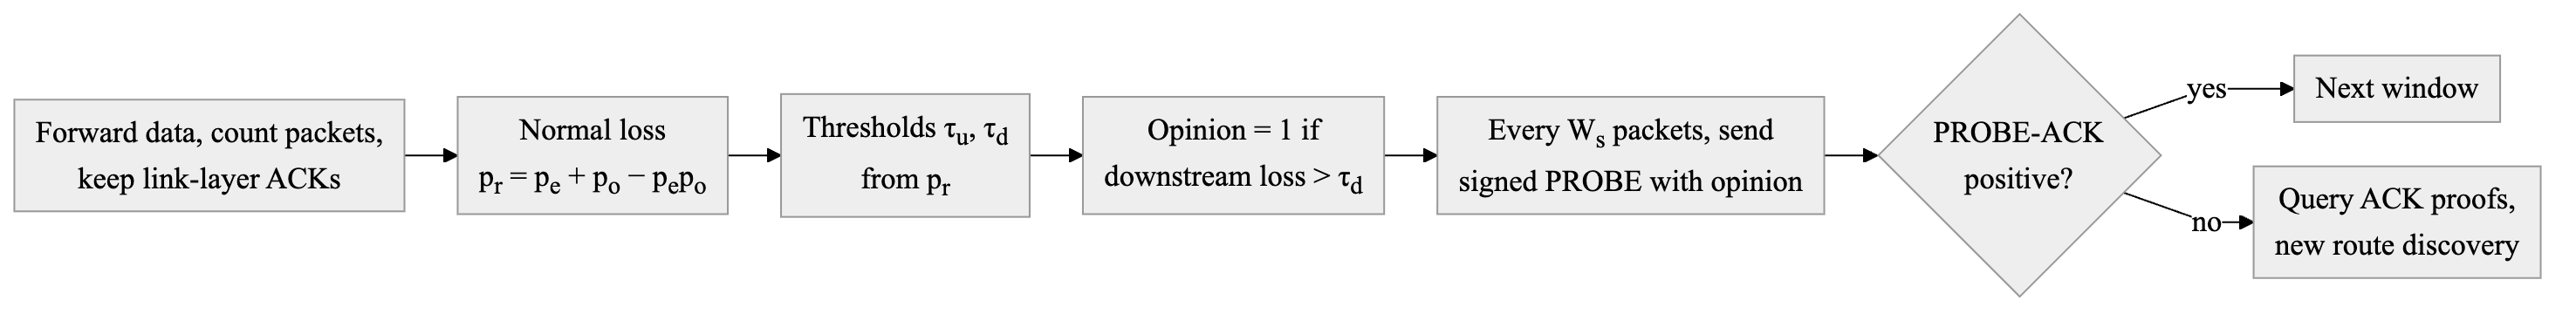
\includegraphics[width=\linewidth,height=2.8cm,keepaspectratio]{figs/fig_cad.png}
\caption{Our flowchart of CAD for one monitored link~\cite{shila2010}.}\label{fig:cad}
\end{figure}

\proscons{Separates normal channel and collision loss from malicious loss. Thresholds come from analysis and follow the channel. Uses upstream and downstream monitoring.}
{Made for mesh routers with link-layer ACKs. PROBE packets, ACK proofs and signatures use energy and channel time. Collisions enter as an average $p_o$, not as a check of each packet.}
{CAD}

\subsection{Attack-resistant trust model ARTMM (2015)}\label{sec:lit-artmm}
\noindent
Han, Jiang, Shu and Guizani state that trust models for terrestrial sensor networks do not suit UASNs, because the acoustic channel is unreliable and the nodes move with the water~\cite{han2015}.
Their model (ARTMM) combines link, data and node trust, and includes channel unreliability and mobility.
They report better accuracy and lower energy use than conventional trust models.
Our description follows the published abstract (Figure~\ref{fig:artmm}).

\begin{figure}[!htb]
\centering
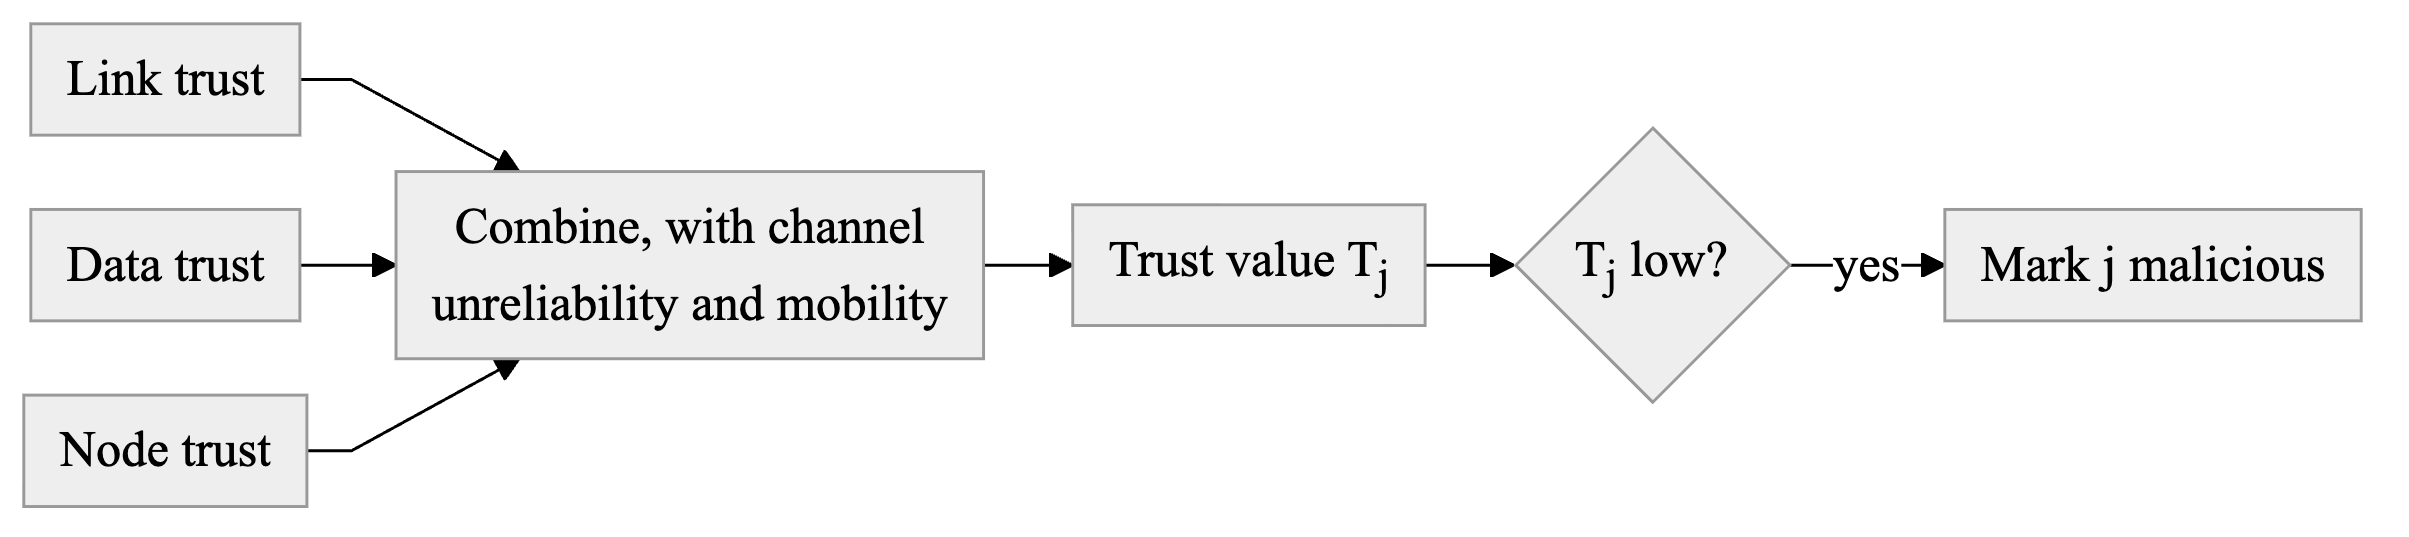
\includegraphics[width=\linewidth,height=2.4cm,keepaspectratio]{figs/fig_artmm.png}
\caption{Our diagram of ARTMM for one neighbour $j$~\cite{han2015}.}\label{fig:artmm}
\end{figure}

\proscons{The first trust model made for the underwater channel and node mobility. Three kinds of evidence make it harder for one attack to fool the model.}
{A poor link can decrease the trust of an honest node. Liu et al.\ report that low link quality has a large effect on ARTMM~\cite{liu2024}.}
{ARTMM}

\subsection{Selective forwarding detection in UnetStack3 (2021)}\label{sec:lit-brc}
\noindent
Dr.~B.~R.~Chandavarkar and N.~Suresh, of the Wireless Information Networking Group at NITK Surathkal, showed a selective forwarding attack and its detection in UnetStack3~\cite{brc2021}.
In a four-node network, the malicious relay takes the address of the honest relay and drops a packet when a random number is above a threshold.
The destination is the only monitor.
A missing packet increases $\beta$, a packet with a wrong destination increases $\alpha$, and a counter above its threshold raises an alarm.
A low packet rate and random node sleep prevent collisions (Figure~\ref{fig:brc}).

\begin{figure}[!htb]
\centering
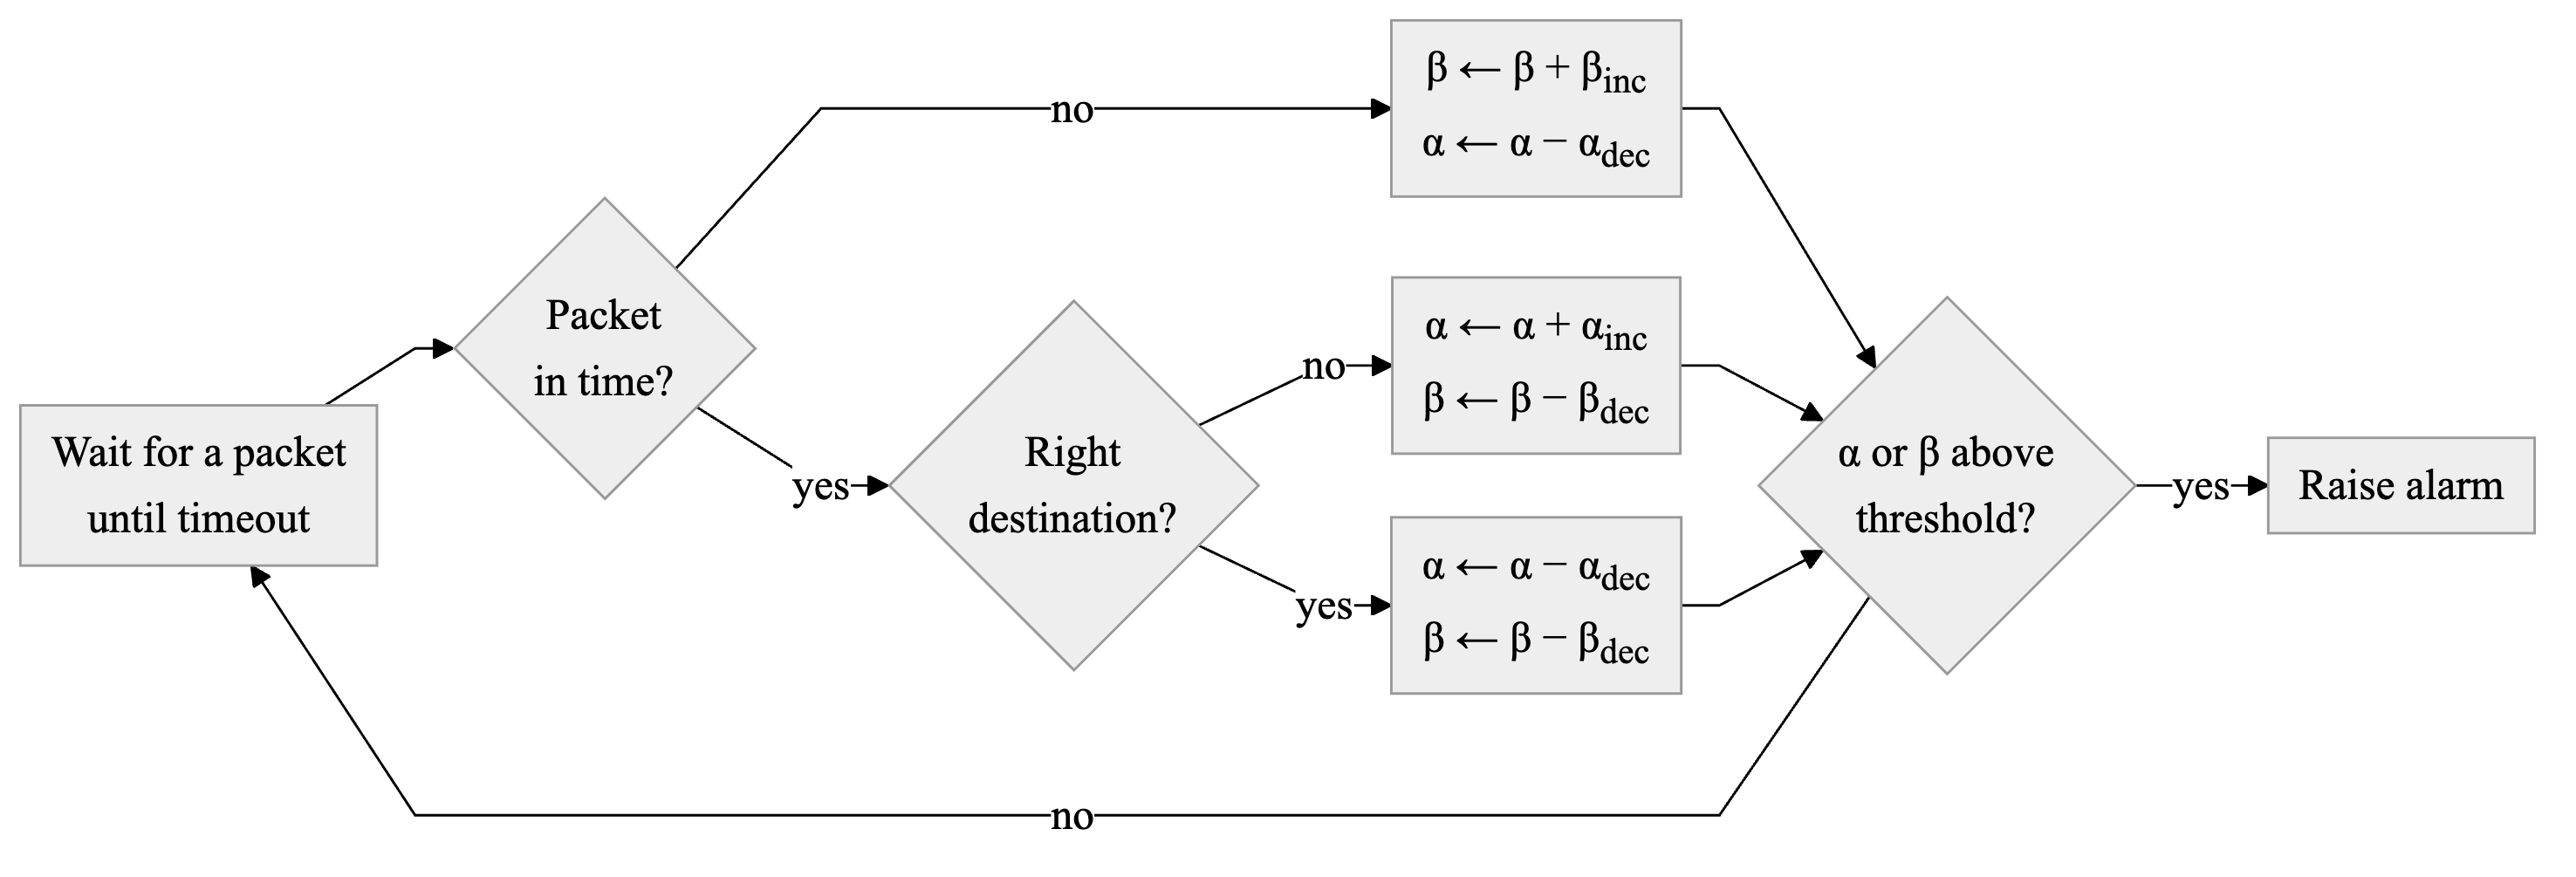
\includegraphics[width=\linewidth,height=4.0cm,keepaspectratio]{figs/fig_brc.png}
\caption{Our flowchart of the counter-based detector at the destination~\cite{brc2021}.}\label{fig:brc}
\end{figure}

\proscons{First demonstration of the attack and its detection in UnetStack3, whose agents can run on real modems. Very light, with one monitor and two counters.}
{The authors state that the alarm does not tell which node attacks or how many. Simple topology, fixed thresholds, and a natural loss also increases $\beta$.}
{the UnetStack3 detector}

\subsection{Trust-aware fuzzy layering routing TAFLRLR (2023)}\label{sec:lit-taflrlr}
\noindent
Han, Du, Wang, Liu and Tian proposed a trust-aware routing protocol with fuzzy logic and layers (TAFLRLR) for UASNs~\cite{han2023}.
HELLO packets give each node a layer, which is its hop count to the sink.
A node selects its next hop from the neighbours that are one layer nearer to the sink.
Direct trust comes from HELLO forwarding, DATA forwarding and residual energy.
A DATA forward that the node does not hear within the round-trip time is abnormal.
Indirect trust from common neighbours and a fuzzy controller give a forwarding probability for each candidate (Algorithm~\ref{alg:taflrlr}).
The authors evaluated it in NS-3.

\begin{algorithm}[!htb]
\caption{Next-hop selection in TAFLRLR~\cite{han2023}}\label{alg:taflrlr}
\footnotesize
\begin{algorithmic}[1]
\State Set the layer of each node by HELLO flooding from the sink
\For{each neighbour $j$ one layer nearer to the sink}
  \State $t_H, t_D \gets (\mathit{normal}+1)/(\mathit{normal}+\mathit{abnormal}+2)$ for HELLO and DATA forwarding; $t_E \gets$ residual energy ratio
  \State $\mathit{DTV}_j \gets$ fuzzy evaluation of $(t_H, t_D, t_E)$; \ $\mathit{ITV}_j \gets$ mean trust from common neighbours
  \State $\mathit{CTV}_j \gets a\,\mathit{DTV}_j + b\,\mathit{ITV}_j$; \ $\mathit{FP}_j \gets$ fuzzy controller(node density of $j$, $\mathit{CTV}_j$)
\EndFor
\State Forward to the candidate with the highest $\mathit{FP}_j$
\end{algorithmic}
\end{algorithm}

\proscons{Trust goes directly into the route selection, so no separate response step is necessary. Layers prevent void areas. Indirect trust uses the view of several neighbours.}
{A DATA forward that is not heard in time counts as abnormal, whatever caused the silence. The paper does not give the trust weights. The trust test uses a nine-node topology.}
{TAFLRLR}

\subsection{Adaptive trust evaluation model ATEM (2024)}\label{sec:lit-atem}
\noindent
Liu, Ye, An and Jiang proposed an adaptive trust evaluation model (ATEM) for abnormal nodes in UASNs~\cite{liu2024}.
It stops a trust cycle when the link score is low, and else combines three kinds of trust (Algorithm~\ref{alg:atem}).
The authors evaluated it in MATLAB with mobile nodes and report better detection than an earlier model on unstable links.

\begin{algorithm}[!htb]
\caption{One trust cycle of ATEM~\cite{liu2024}}\label{alg:atem}
\footnotesize
\begin{algorithmic}[1]
\State $L \gets$ link score from receptions, with more weight on recent ones; \textbf{if} $L < \varepsilon$, stop this cycle
\State Communication trust from successes and failures; data trust from deviation; energy trust
\State Direct trust $\gets$ variable-weight fuzzy evaluation, with more weight on a low indicator
\State Remove recommendations that deviate above $\theta$; low combined trust marks an abnormal node
\end{algorithmic}
\end{algorithm}

\proscons{Does not judge a node on an unstable link, which protects honest nodes. Removes dishonest recommendations. Includes node mobility.}
{The link check is for a full cycle and a full link, so a silence inside a good cycle still counts as a failure. Evaluated in MATLAB, without a network stack.}
{ATEM}

\subsection{Comparison of the approaches}\label{sec:lit-compare}
\noindent
Table~\ref{tab:compare} compares the approaches.
The counter methods need few or no extra packets, but they count every silence as a drop.
CAD and the trust models consider link quality, but as an average value for a link or a cycle.
From this comparison we find three gaps.
\textbf{G1.} No approach checks, for each watched packet, whether the monitor was able to hear the forward.
\textbf{G2.} Only CAD sets a normal loss for each link, and it needs probes and ACK proofs, which are expensive under water.
\textbf{G3.} The UnetStack3 detector uses one monitor and does not name the attacker.

\begin{table}[!htb]
\centering\footnotesize\setlength{\tabcolsep}{3pt}
\caption{Comparison of the reviewed approaches.}\label{tab:compare}
\begin{tabular}{>{\raggedright\arraybackslash}p{2.2cm} >{\raggedright\arraybackslash}p{1.7cm} >{\raggedright\arraybackslash}p{2.3cm} >{\raggedright\arraybackslash}p{2.8cm} >{\raggedright\arraybackslash}p{2.9cm} >{\raggedright\arraybackslash}p{2.3cm}}
\toprule
Approach & Network & Monitor & Normal loss & Forward the monitor could not hear & Output \\
\midrule
Watchdog~\cite{marti2000} & Ad hoc & Sender & Not used & Counts as a failure & Report to source \\
Two-hop~\cite{hai2008} & Sensor & Neighbours & Not used & Alert $\alpha$ & Alerts to source \\
CAD~\cite{shila2010} & Mesh & Up/downstream & Per link, channel and collisions & Inside the average $p_o$ & Node, new route \\
ARTMM~\cite{han2015} & Underwater & Each node & Link trust metric & No check in the abstract & Trust value \\
UnetStack3~\cite{brc2021} & Underwater & Destination & Not used & Increases $\beta$ & Alarm only \\
TAFLRLR~\cite{han2023} & Underwater & Sender & Not used & Counts as abnormal & Next-hop choice \\
ATEM~\cite{liu2024} & Underwater & Each node & Link score per cycle & Cycle skipped, else a failure & Trust value \\
\midrule
Ours & Underwater & Neighbours & Per link, distance and area & Window excluded & Ranked suspects \\
\bottomrule
\end{tabular}
\end{table}

%==========================================================
\section{Proposed approach}\label{sec:prop}
\noindent
Every node watches every relay that it overhears, and counts a window only when it was able to observe the forward (G1).
The sink compares the forwards heard with the forwards expected on each link (G2), and ranks the suspects from all monitors (G3), as Figure~\ref{fig:arch} shows.

\begin{figure}[H]
\centering
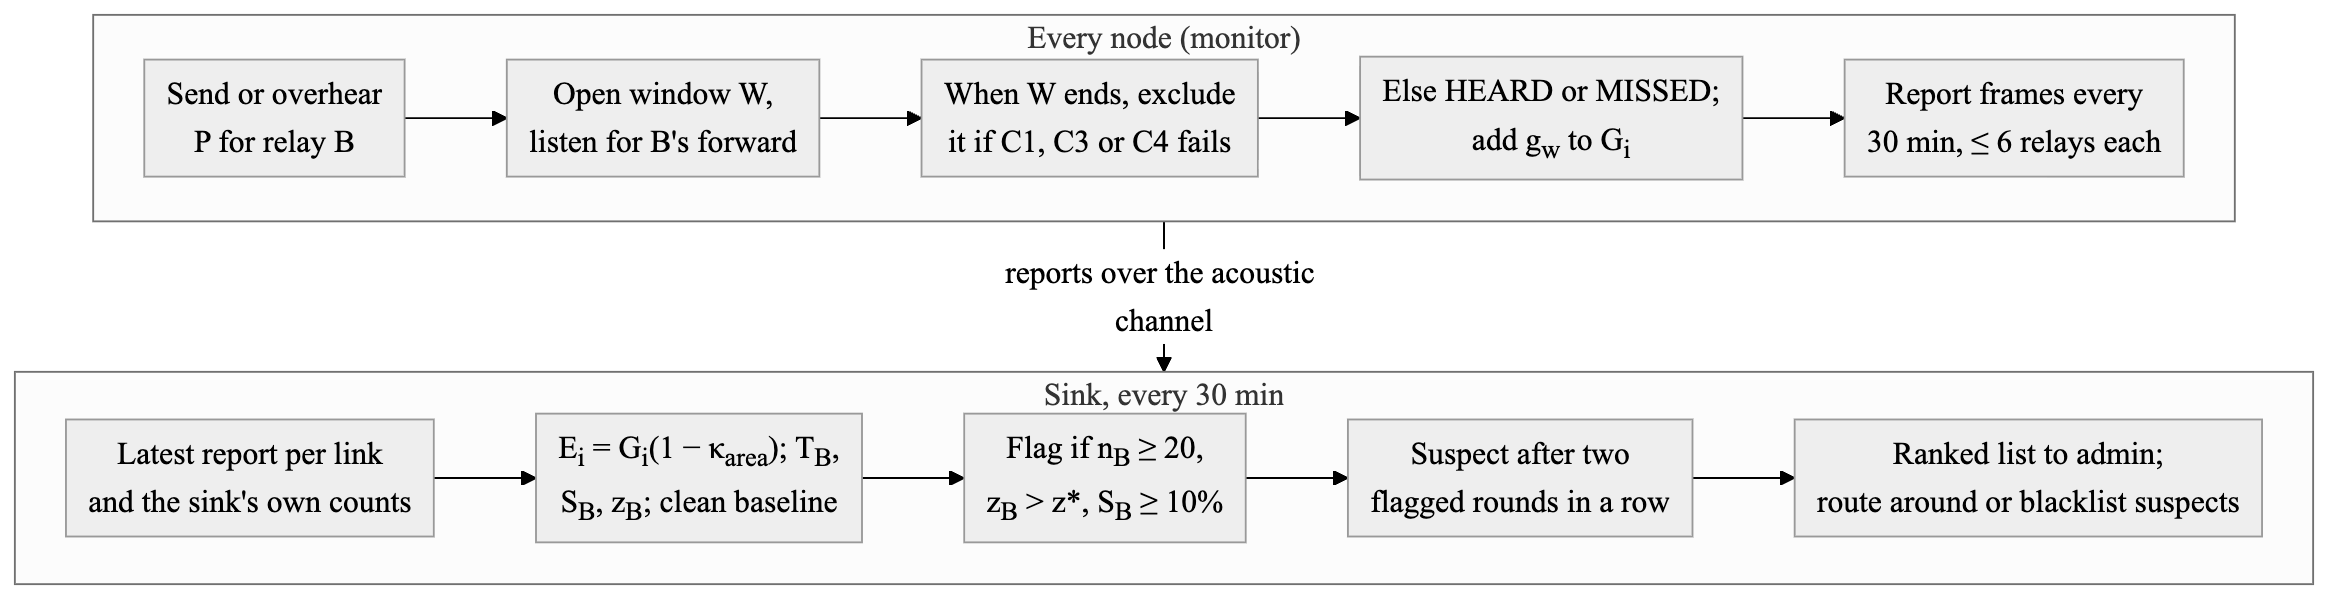
\includegraphics[width=\linewidth,height=4.0cm,keepaspectratio]{figs/fig_arch_final.png}
\caption{Architecture of the proposed detector.}\label{fig:arch}
\end{figure}

\subsection{System and attack model}\label{sec:prop-model}
\noindent
Twenty static sensors and one sink are in a 4~km by 4~km field with a 1500~m range.
Each sensor sends to the nearest neighbour that is one hop nearer to the sink.
Nodes know the positions, the speed of sound $c$ and the frame loss $e(d) = 0.15\,(d/1500)^2$ at distance $d$.
The busiest one, two or three relays are grayholes.
A grayhole drops each packet that it must forward with probability $p$, and it still sends its own data and reports.
Monitors report truthfully, and grayholes do not collude.

\subsection{Observability filter (G1)}\label{sec:prop-filter}
\noindent
Let $M$ be the monitor, $A$ the sender of packet $P$ and $B$ the relay.
$M$ receives the end of the frame of $A$ at time $t$. It then calculates the interval $I_B$ in which $P$ arrived at $B$, and the window $W$ for the forward of $B$:
\begin{gather}
t_A = t - \tfrac{d(A,M)}{c},\qquad
I_B = \bigl[t_A + \tfrac{d(A,B)}{c} - T_f,\ e_B\bigr],\quad e_B = t_A + \tfrac{d(A,B)}{c},\\
W = \bigl[e_B + \tfrac{d(B,M)}{c},\ e_B + T_w + T_f + \tfrac{d(B,M)}{c}\bigr].
\end{gather}
The frame time is $T_f \approx 1.02$~s.
The forward allowance $T_w = 2$~s is the time that a relay can hold a packet before it forwards it.
$M$ keeps a window only if three conditions are true.
\textbf{C1:} $M$ did not transmit during $W$.
\textbf{C3:} $M$ did not hear $B$ transmit during $I_B$.
\textbf{C4:} no frame known to $M$ arrived at $B$ during $I_B$, where a frame of node $C$ arrives at $B$ after $d(C,B)/c$.
A kept window is HEARD or MISSED, and an excluded window counts as neither.
A corrupted frame at $M$ does not exclude a window, because the forward of $B$ can cause it, but a drop cannot.
If the filter excluded such windows, it would remove more forwards than drops.

\subsection{Expected forwards and trust (G2)}\label{sec:prop-trust}
\noindent
Let $g_w = (1-e(d_{AB}))(1-e(d_{BM}))$ be the probability that an honest forward reaches $M$ on the channel alone.
For each monitor and relay link $i$, let $n_i$ be the kept windows, $O_i$ the heard forwards and $G_i = \sum_w g_w$.
Collisions that $M$ cannot see remove more forwards, so link $i$ has a residual loss $\kappa_i = \max(0,\, 1 - O_i/G_i)$.
We use $\kappa_i$ only when $n_i \geq 5$.
We sort the links into near, medium and far areas by length.
For relay $B$, the normal residual loss of an area is the median $\kappa$ of the links of the other relays in that area, so $B$ cannot increase its own baseline. Then
\begin{equation}
E_i = G_i\bigl(1-\kappa_{\mathrm{area}(i),\,-B}\bigr), \qquad
T_B = \frac{\sum_i O_i}{\sum_i E_i}, \qquad
S_B = 100\,\max(0,\, 1 - T_B).
\end{equation}
$T_B$ is the average of the trust $O_i/E_i$ of each monitor, weighted by $E_i$.
If $E_i$ is correct and $B$ keeps each packet with probability $1-p$, the expected value of $O$ is $(1-p)E$.
Thus $S_B$ estimates the drop rate in percent.

\subsection{Decision, confirmation and response (G3)}\label{sec:prop-decision}
\noindent
The shortfall of $B$ is $z_B = (\sum E_i - \sum O_i)/\sqrt{\sum E_i \max(0.01,\, 1 - E_i/n_i)}$.
Monitors that watch the same packet are correlated, so we divide $z_B$ by $\sqrt{\phi}$.
Here $\phi = \max(1, m/0.455)$, and $m$ is the median $z_B^2$ of the relays with $z_B < 0$.
For $k$ judged relays, the threshold is $z^* = \Phi^{-1}(1-\alpha/k)$.
The tuning parameter $\alpha$ is set on networks that we do not use for the test.
Grayholes in one area increase its median and hide one another.
Thus the sink removes confirmed suspects and relays with $n_B \geq 20$ and $S_B \geq 10$ from the baseline, and calculates the estimate again (Algorithm~\ref{alg:sink}).
Reports are cumulative, so a lost report only delays evidence.
The sink gives the administrator the ranked list.
The default response sends traffic around each suspect where another path exists.
A stronger response blacklists the suspects, and Section~\ref{sec:res-blacklist} tests it.

\begin{algorithm}[H]
\caption{Decision at the sink, every 30 minutes}\label{alg:sink}
\footnotesize
\begin{algorithmic}[1]
\State $R \gets$ latest delivered report of each link, plus the counters of the sink; $X \gets$ confirmed suspects
\Repeat \Comment{baseline cleaning, at most 3 times}
  \State For each relay $B$: $E_i \gets G_i(1-\mathrm{median}\{\kappa_j : j \text{ in the same area}, \mathrm{relay}(j) \notin X \cup \{B\}\})$; calculate $T_B$, $S_B$, $z_B$
  \State Divide each $z_B$ by $\sqrt{\phi}$; \ $X \gets$ confirmed suspects $\cup \{B : n_B \geq 20,\ S_B \geq 10\}$
\Until{$X$ does not change}
\State $F \gets \{B : n_B \geq 20,\ S_B \geq 10,\ z_B > z^*\}$
\State $\mathit{suspects} \gets \mathit{suspects} \cup (F \cap F_{\mathrm{previous}})$; \ $F_{\mathrm{previous}} \gets F$
\State Give the administrator the relays ranked by $S_B$; apply the response to $\mathit{suspects}$
\end{algorithmic}
\end{algorithm}

\subsection{Worked example}\label{sec:prop-example}
\noindent
Two monitors watch relay $B$, and the normal residual loss of their area is $\kappa = 0.10$.
Monitor 1 kept $n_1 = 200$ windows with $G_1 = 180$, so $E_1 = 180 \times 0.90 = 162$.
Monitor 2 kept $n_2 = 100$ windows with $G_2 = 85$, so $E_2 = 76.5$.
If $B$ is a grayhole, monitor 1 hears $O_1 = 113$ forwards and monitor 2 hears $O_2 = 54$.
Then $T_B = 167/238.5 = 0.70$ and $S_B = 30.0\%$.
The shortfall is $z_B = (238.5 - 167)/\sqrt{162 \times 0.19 + 76.5 \times 0.235} = 71.5/6.98 = 10.2$.
With $k = 10$ judged relays and $\alpha = 10^{-4}$, the threshold is $z^* = \Phi^{-1}(1 - 10^{-5}) = 4.26$.
Thus $B$ is flagged, because $n_B = 300 \geq 20$, $S_B \geq 10$ and $z_B > z^*$.
If the sink flags $B$ again in the next round, it confirms $B$ as a suspect.
If $B$ is honest, the monitors hear approximately the expected forwards, for example $O_1 = 160$ and $O_2 = 75$.
Then $T_B = 0.985$ and $S_B = 1.5\%$, which is less than 10\%, so the sink does not flag $B$.

\subsection{Justification}\label{sec:prop-justify}
\begin{itemize}\setlength{\itemsep}{0pt}\setlength{\parskip}{0pt}\setlength{\topsep}{2pt}
\item \textbf{Filter before outcome.} C1, C3 and C4 use only times that $M$ records. They apply to heard and missed forwards in the same way, so the filter does not prefer either result.
\item \textbf{Expectation without probes.} Positions and the loss curve give $G_i$, and the other relays give the residual loss, so no extra packets are necessary. The median ignores a few bad links, so the lossy links of a grayhole do not increase the normal loss of its area.
\item \textbf{Cleaning and confirmation.} Several grayholes in one area increase its normal loss and hide one another, so cleaning removes them from the baseline. A suspect needs two flagged rounds, so one noisy round cannot cause an accusation.
\item \textbf{Few false accusations.} Each honest relay that a detector accuses has a cost. If the sink blacklists it, the nodes behind it can lose their only path. Thus a detector for this network must keep false accusations near zero.
\end{itemize}

%==========================================================
\section{Implementation}\label{sec:impl}

\subsection{Tools and environment}\label{sec:impl-tools}
\noindent
We implemented the detector in UnetStack 7.0.0, community edition, on Java~8~\cite{chitre2014}.
The agents and the simulation scripts are in Groovy.
The agent of each node subscribes to the physical-layer notifications of UnetStack~\cite{unethandbook}.
\texttt{TxFrameNtf} arrives when the node transmits a frame.
\texttt{RxFrameNtf} arrives when the node decodes a frame, also a frame for another node.
Python with matplotlib draws the graphs.
The script \texttt{run.sh} runs four steps.
\texttt{record.groovy} records the counters of every monitor.
\texttt{compare.groovy} replays the decisions of the sink for every method on the same counters.
\texttt{network.groovy} runs the live network with reports and responses.
\texttt{analysis/plots.py} and \texttt{analysis/final\_figs.py} draw the graphs.

\subsection{Class diagram}\label{sec:impl-classes}
\noindent
Figure~\ref{fig:classes} shows the classes and how the simulation scripts use them.
\texttt{MonitorNode} extends the \texttt{UnetAgent} class of UnetStack.
\texttt{DistanceLossChannel} extends the \texttt{ProtocolChannelModel} class.
\texttt{Detectors} holds the three detection methods as static functions, so every method reads the same evidence.
The scripts \texttt{record.groovy} and \texttt{network.groovy} create the \texttt{MonitorNode} agents, and \texttt{network.groovy} and \texttt{compare.groovy} call \texttt{Detectors}.

\begin{figure}[htbp]
\centering
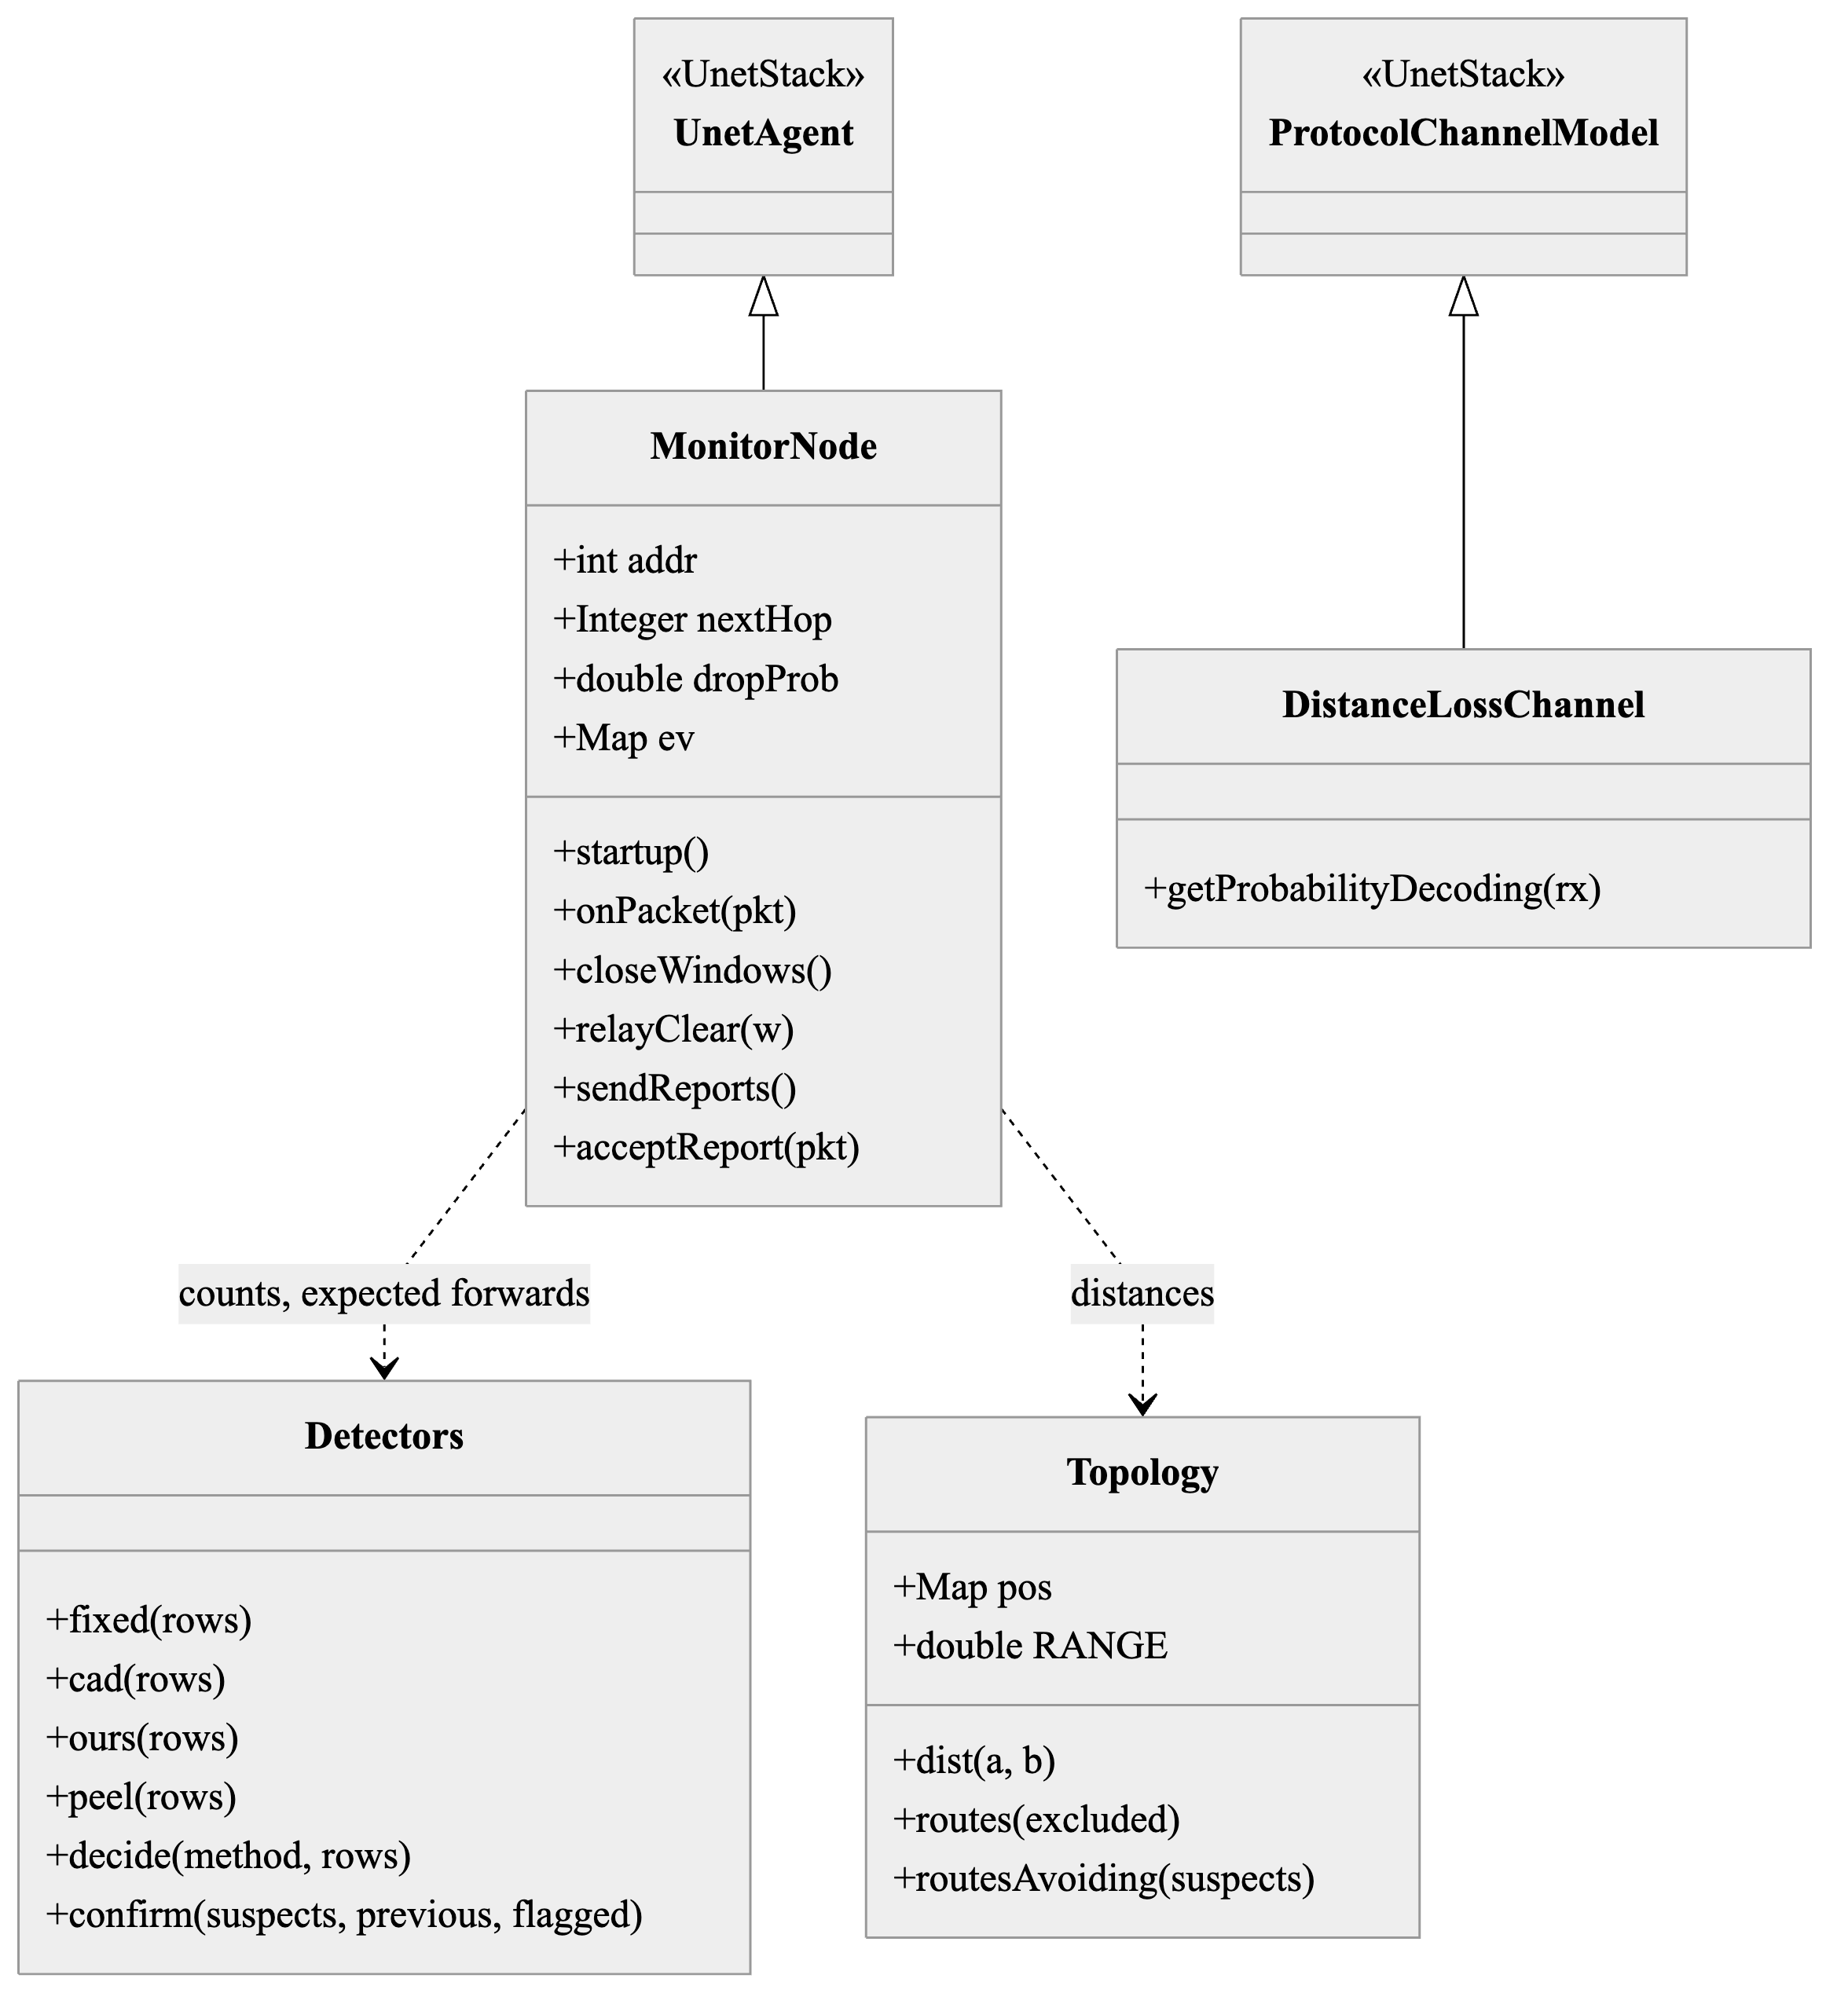
\includegraphics[width=0.62\linewidth]{figs/classes.png}
\caption{Class diagram, drawn with Mermaid. Open arrow heads show inheritance, and dashed arrows show use.}\label{fig:classes}
\end{figure}

\subsection{Node agent and the attack}\label{sec:impl-agent}
\noindent
\texttt{startup()} starts each node.
It finds the physical-layer agent, subscribes to its notifications and adds three behaviours.
The first behaviour is a Poisson generator for the data of the node.
The second is a 200~ms ticker that closes the windows that ended.
The third is a 30-minute ticker for the checkpoint.
A data packet has 8 bytes: origin, sequence number, generation time and hop count.
\texttt{onPacket()} contains the attack (Algorithm~\ref{alg:onpacket}).
The sink records deliveries and keeps reports.
Every other node forwards the packet, unless it is a grayhole and the random draw selects a drop.

\begin{algorithm}[htbp]
\small
\caption{\texttt{startup()} and \texttt{onPacket()} in \texttt{MonitorNode}}\label{alg:onpacket}
\begin{algorithmic}[1]
\Function{startup}{}
  \State $\mathit{phy} \gets$ agent for the PHYSICAL service; subscribe to its topic and to DATAGRAM
  \State Add PoissonBehavior($1/\mathit{genRate}$) that calls \textsc{generate}
  \State Add TickerBehavior(200 ms) that calls \textsc{closeWindows}
  \State Add TickerBehavior(30 min) that calls \textsc{snapshot}, \textsc{sendReports} and, at the sink, \textsc{onRound}
\EndFunction
\Function{onPacket}{$\mathit{pkt}$}
  \If{this node is the sink}
    \If{$\mathit{pkt}$ is a report} \State \textsc{acceptReport}($\mathit{pkt}$) \Else \State record delivery and latency \EndIf
    \State \Return
  \EndIf
  \If{$\mathit{dropProb} > 0$ \textbf{and} random() $< \mathit{dropProb}$} \State \Return \Comment{grayhole drops the packet} \EndIf
  \State $\mathit{pkt}.\mathit{hops} \gets \mathit{pkt}.\mathit{hops}+1$; \textsc{transmit}($\mathit{pkt}$) to $\mathit{nextHop}$
\EndFunction
\end{algorithmic}
\end{algorithm}

\subsection{Watch windows and the observability check}\label{sec:impl-windows}
\noindent
\texttt{processMessage()} receives the notifications.
When the node transmits a frame, it records the transmission interval and opens a window for its next hop.
When it decodes a frame for another node, it records the transmission interval of the sender.
It then marks a matching open window as heard and opens a window for the destination of the frame.
\texttt{closeWindows()} and \texttt{relayClear()} apply C1, C3 and C4 (Algorithm~\ref{alg:close}).
Each result goes into one of 32 counter bins.
The bins record if the monitor was the sender, which conditions failed and if the monitor heard the forward.
With all 32 bins, the same evidence supplies the fixed watchdog (sender windows only), the CAD-style detector and our detector with and without the filter.

\begin{algorithm}[htbp]
\small
\caption{\texttt{closeWindows()} and \texttt{relayClear()} in \texttt{MonitorNode}}\label{alg:close}
\begin{algorithmic}[1]
\Function{closeWindows}{}
  \For{each window $w$ with now $> \mathrm{end}(W) + 50$ ms}
    \State $c_{13} \gets$ not overlaps($\mathit{myTx}$, $W$) \textbf{and} not overlaps($\mathit{heardTx}[B]$, $I_B$)
    \State $c_2 \gets$ not overlaps($\mathit{badFrames}$, $W$) \Comment{recorded, not used by our detector}
    \State $c_4 \gets$ \textsc{relayClear}($w$)
    \State $i \gets$ idx($\mathit{sender}, c_{13}, c_2, c_4, \mathit{heard}$); \; $\mathit{ev}[B][i] \gets \mathit{ev}[B][i] + 1$
    \State $\mathit{expect}[B][i] \gets \mathit{expect}[B][i] + (1-e(d(A,B)))(1-e(d(B,M)))$
    \State Remove $w$
  \EndFor
\EndFunction
\Function{relayClear}{$w$}
  \For{each node $C \notin \{A, B\}$ with known frames and $d(C,B) \leq$ range}
    \State $s \gets d(C,B)/c$
    \If{a frame $[t_0,t_1]$ of $C$ has $[t_0+s, t_1+s]$ that overlaps $I_B$} \State \Return false \EndIf
  \EndFor
  \State \Return true
\EndFunction
\end{algorithmic}
\end{algorithm}

\subsection{Reports and the decision at the sink}\label{sec:impl-reports}
\noindent
At each checkpoint, a node freezes its counters and puts them into one report frame.
The frame has a 12-byte header: the 8-byte packet header and a 32-bit busy fraction.
Each watched relay adds one 17-byte entry: relay identifier, two 32-bit counts and a 64-bit expected-forward sum.
Up to six entries (114 bytes) fit into the 128-byte data frame of the simulator.
Nodes send their reports at random times in the ten minutes after the checkpoint, to decrease collisions between reports.
Reports go to the sink like data, so the channel can lose them and a grayhole can drop them.
\texttt{acceptReport()} rejects incorrect entries, duplicates and reports older than the report that the sink has.
The sink keeps the latest delivered report of each link.

\texttt{Detectors.ours()} calculates the trust and the shortfall of Section~\ref{sec:prop-trust} and Section~\ref{sec:prop-decision}.
\texttt{peel()} repeats it for baseline cleaning, and \texttt{confirm()} applies the two-round rule.
After each round, the sink calls \texttt{routesAvoiding()}.
This function gives each node the shortest route that does not use a suspect.
A node with no such route keeps its old route.
For blacklisting, \texttt{routes(excluded)} removes the suspects from the network, so a node without another path loses its route.

\subsection{Baselines and channel}\label{sec:impl-baselines}
\noindent
The two baselines use the same agent, reports, confirmation and response, so only the detection rule is different.
The fixed watchdog uses sender windows and accuses a relay when its miss rate is more than 30\%.
The CAD-style detector uses sender windows with the normal loss $p_r = 1-(1-e(d))^2(1-p_o)^2$.
Here $p_o = 1-(1-R_b)^2$ comes from the busy ratio $R_b$ of the monitor.
It flags a relay when a pooled binomial $z$ is more than 2.
\texttt{DistanceLossChannel} changes one method of the protocol channel model.
A frame at distance $d$ then decodes with probability $1-0.15\,(d/1500)^2$.
The command \texttt{./run.sh demo} runs one live network with three grayholes in approximately three minutes and prints the ranked suspect list.
The command \texttt{./run.sh} makes all numbers and graphs again in approximately one hour.

%==========================================================
\section{Results and analysis}\label{sec:results}

\subsection{Simulation parameters}\label{sec:res-params}
\noindent
Table~\ref{tab:params} gives the parameters of all runs.

\begin{table}[htbp]
\centering\small
\caption{Simulation parameters.}\label{tab:params}
\begin{tabular}{>{\raggedright\arraybackslash}p{3.4cm} >{\raggedright\arraybackslash}p{11.4cm}}
\toprule
Parameter & Value \\
\midrule
Simulator & UnetStack 7.0.0 community edition, Java 8 \\
Channel & Protocol channel model, range 1500 m, decoding probability $1-0.15(d/1500)^2$ \\
Sound speed, frame & 1500 m/s; 128-byte data frame of approximately 1.02 s \\
Network, routing & 20 sensors and one sink in 4 km $\times$ 4 km at 50 m depth; shortest hop count \\
Traffic, grayholes & Poisson, 0.001 to 0.01 packets/s per sensor (0.005 default); 1 to 3 busiest relays drop 30\% \\
Timing & $T_w = 2$ s; decision every 30 min; 6 h recorded runs and 12 h live runs \\
Networks & Tuning topologies 101 to 106; test topologies 201 to 210 \\
Own thresholds & Fixed watchdog miss rate $> 0.3$; CAD-style $z > 2$; ours $\alpha = 10^{-4}$ \\
Responses & Route around suspects where another path exists; or blacklist the suspects \\
\bottomrule
\end{tabular}
\end{table}

\subsection{Scenarios}\label{sec:res-scenarios}
\noindent
The recorded runs have eight scenarios on each test topology.
\emph{Load} has one 30\% grayhole at four traffic loads, and each load also has a run with no attacker.
\emph{Drop} has one grayhole that drops 10, 20, 50 or 100\%.
\emph{Two} and \emph{three} make the two or three busiest relays grayholes.
\emph{Near} attacks the relay with the nearest neighbours.
In \emph{hotspot}, three well-connected sensors send six times more traffic than the others, with the same total traffic.
\emph{Large} has 40 sensors in 6~km by 6~km, and \emph{sparse} has 20 sensors in 5~km by 5~km.
The 12-hour live network adds reports, detection and the response.
It has four attack settings: one grayhole at loads 0.005 and 0.01, and two and three grayholes at load 0.005.
We ran each setting once with route changes and once with blacklisting.

\subsection{Performance metrics}\label{sec:res-metrics}
\noindent
An honest sensor is a sensor that is not a grayhole.
We use four metrics.
\begin{itemize}\setlength{\itemsep}{0pt}
  \item \textbf{Delivery ratio.} The percentage of the data packets generated by honest sensors that arrive at the sink:
  \[
  \text{Delivery ratio} = 100 \times \frac{\text{honest data packets received at the sink}}{\text{honest data packets generated}}\ \%.
  \]
  The data of the grayholes is not included. Report frames use the same channel, but they are not data packets.
  \item \textbf{Grayholes caught.} The percentage of grayholes that are confirmed suspects at the end of a run.
  \item \textbf{Honest relays accused.} The number of honest relays that are confirmed suspects at the end of a run.
  \item \textbf{Detection time.} The time until the detector confirms every grayhole.
\end{itemize}
\noindent
A difference between two delivery ratios is absolute.
For example, a change from 40.0\% to 50.0\% is an absolute increase of 10.0\%.
A topology is the independent unit.
All intervals are 95\% $t$-intervals over the ten test topologies, and we pair two methods by topology.

\subsection{Summary of the results}\label{sec:res-summary}
\noindent
Table~\ref{tab:summary} gives the main numbers.
The subsections after it give the graph and the details for each row.

\begin{table}[htbp]
\centering\small
\caption{Summary of the results. The last column gives the subsection with the details.}\label{tab:summary}
\begin{tabular}{>{\raggedright\arraybackslash}p{6.4cm} c c c c}
\toprule
Result & \shortstack{Fixed\\watchdog} & CAD-style & \textbf{Ours} & Details \\
\midrule
Delivery ratio with blacklisting (no defence: 45.6\%) & 23.2\% & 46.8\% & \textbf{45.7\%} & \ref{sec:res-blacklist} \\
Honest relays blacklisted per run & 4.45 & 0.72 & \textbf{0.28} & \ref{sec:res-blacklist} \\
Honest relays accused per run, no attacker, highest load & 6.2 & 0.7 & \textbf{0.1} & \ref{sec:res-false} \\
Estimated drop rate for a true drop rate of 50\% & n/a & 31.3\% & \textbf{47.2\%} & \ref{sec:res-list} \\
\bottomrule
\end{tabular}
\end{table}

\subsection{Delivery ratio with blacklisting}\label{sec:res-blacklist}
\noindent
In this test, the sink blacklists each confirmed suspect, so no node uses it as a relay.
Figure~\ref{fig:blacklist}(a) gives the mean delivery ratio over the four attack settings.
With the fixed watchdog, the delivery ratio is 23.2\%.
With our detector, it is 45.7\%.
The mean of the paired differences is an absolute increase of 22.6\%, with a 95\% interval of $\pm 7.9\%$.
Our detector gives a higher delivery ratio in 38 of the 40 runs.
Table~\ref{tab:blacklist} gives the delivery ratio for each setting.
The increase over the fixed watchdog is 17.7\% to 27.5\% in each setting.

\begin{figure}[htbp]
\centering
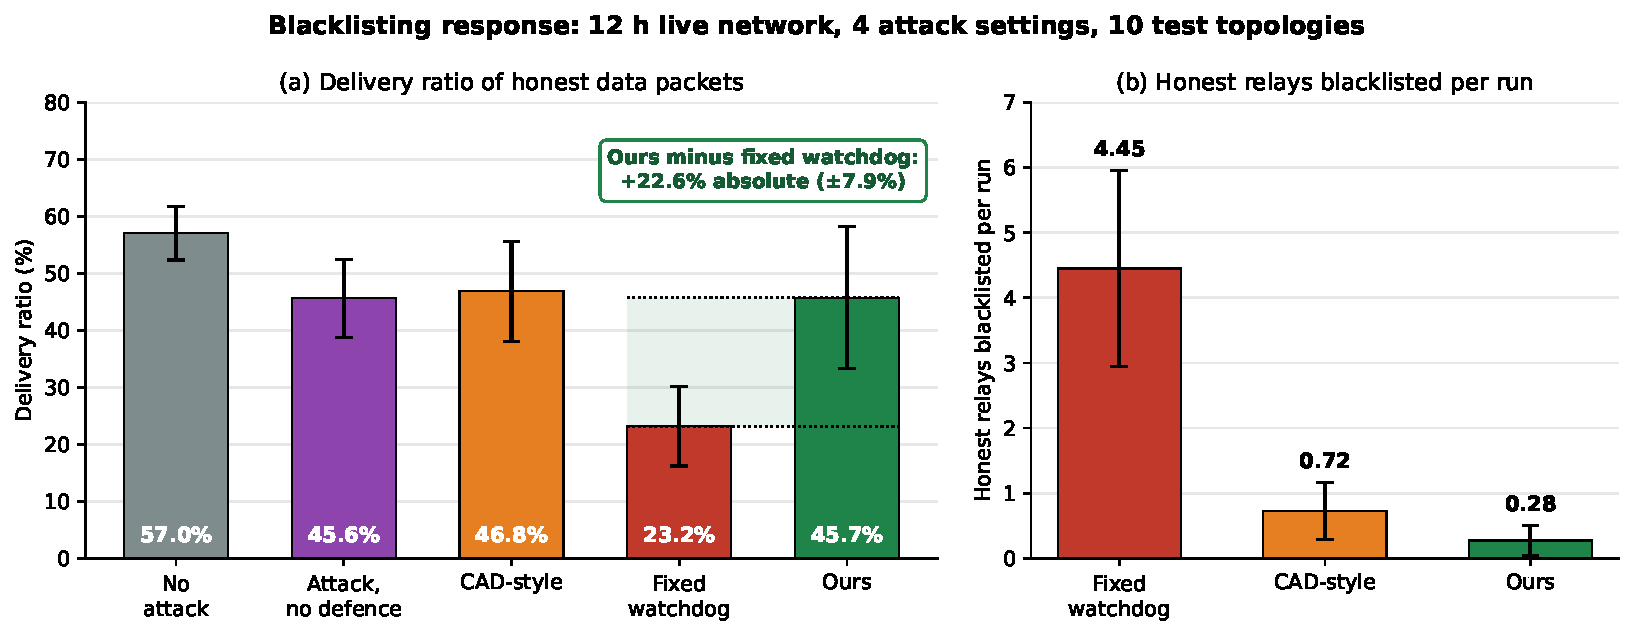
\includegraphics[width=\linewidth]{figs/blacklist.pdf}
\caption{Blacklisting response (12 h live network, four attack settings, ten test topologies, 95\% $t$-intervals). (a) Delivery ratio of honest data packets. The shaded band is the difference between the fixed watchdog and our detector. (b) Honest relays that each detector blacklisted per run.}\label{fig:blacklist}
\end{figure}

\begin{table}[htbp]
\centering\small
\caption{Delivery ratio with blacklisting for each attack setting (mean over ten test topologies). The last column uses the unrounded values.}\label{tab:blacklist}
\begin{tabular}{l c c c c c c}
\toprule
Grayholes, load & No attack & \shortstack{Attack,\\no defence} & CAD-style & \shortstack{Fixed\\watchdog} & \textbf{Ours} & \shortstack{Ours minus\\fixed watchdog} \\
\midrule
1, 0.005 & 60.5\% & 52.1\% & 52.4\% & 24.5\% & \textbf{52.0\%} & 27.5\% \\
1, 0.01 & 48.8\% & 42.9\% & 42.2\% & 17.9\% & \textbf{41.6\%} & 23.7\% \\
2, 0.005 & 59.6\% & 45.4\% & 47.8\% & 24.1\% & \textbf{45.6\%} & 21.5\% \\
3, 0.005 & 59.2\% & 42.2\% & 44.9\% & 26.1\% & \textbf{43.8\%} & 17.7\% \\
\midrule
All settings & 57.0\% & 45.6\% & 46.8\% & 23.2\% & \textbf{45.7\%} & 22.6\% \\
\bottomrule
\end{tabular}
\end{table}

\noindent
The cause of the difference is the false accusations (Figure~\ref{fig:blacklist}(b) and Table~\ref{tab:blacklist-acc}).
The fixed watchdog blacklisted 4.45 honest relays per run.
Each blacklisted honest relay also cuts off the nodes that use it as their only path.
Our detector blacklisted 0.28 honest relays per run and caught 93\% of the grayholes.

\begin{table}[htbp]
\centering\small
\caption{Honest relays blacklisted per run and grayholes caught, with blacklisting (mean over ten test topologies).}\label{tab:blacklist-acc}
\begin{tabular}{l c c c c c c}
\toprule
 & \multicolumn{2}{c}{Fixed watchdog} & \multicolumn{2}{c}{CAD-style} & \multicolumn{2}{c}{\textbf{Ours}} \\
Grayholes, load & Honest & Caught & Honest & Caught & Honest & Caught \\
\midrule
1, 0.005 & 4.1 & 100\% & 0.8 & 60\% & \textbf{0.4} & \textbf{100\%} \\
1, 0.01 & 6.4 & 90\% & 1.2 & 30\% & \textbf{0.6} & \textbf{80\%} \\
2, 0.005 & 3.8 & 100\% & 0.3 & 70\% & \textbf{0.1} & \textbf{100\%} \\
3, 0.005 & 3.5 & 93\% & 0.6 & 67\% & \textbf{0.0} & \textbf{93\%} \\
\midrule
All settings & 4.45 & 96\% & 0.72 & 57\% & \textbf{0.28} & \textbf{93\%} \\
\bottomrule
\end{tabular}
\end{table}

\noindent
This result has two limits.
First, the gain is over the fixed watchdog.
With blacklisting, our delivery ratio (45.7\%) is the same as with no defence (45.6\%) and the same as with the CAD-style detector (46.8\%), within the intervals.
The CAD-style detector keeps its delivery ratio because it accuses few relays, but it caught only 57\% of the grayholes.
Second, blacklisting a correct suspect can also cut off nodes.
On topology 205, a correctly caught grayhole was the only path for many nodes, and our increase over the fixed watchdog is only 1.3\% there.

\subsection{False accusations as traffic increases}\label{sec:res-false}
\noindent
Figure~\ref{fig:fig2} shows why the fixed watchdog fails.
With no attacker, it accused 1.0 honest relay per run at the lowest load and 6.2 at the highest load.
Collisions and half-duplex deafness increase with traffic, and the fixed watchdog counts them as drops.
The CAD-style detector accused 0.3 to 0.7 honest relays per run.
Our detector accused 0 to 0.1, because it excludes the windows that the monitor could not observe.
With one grayhole, the result is almost the same (Figure~\ref{fig:fig2}(b)).

\begin{figure}[htbp]
\centering
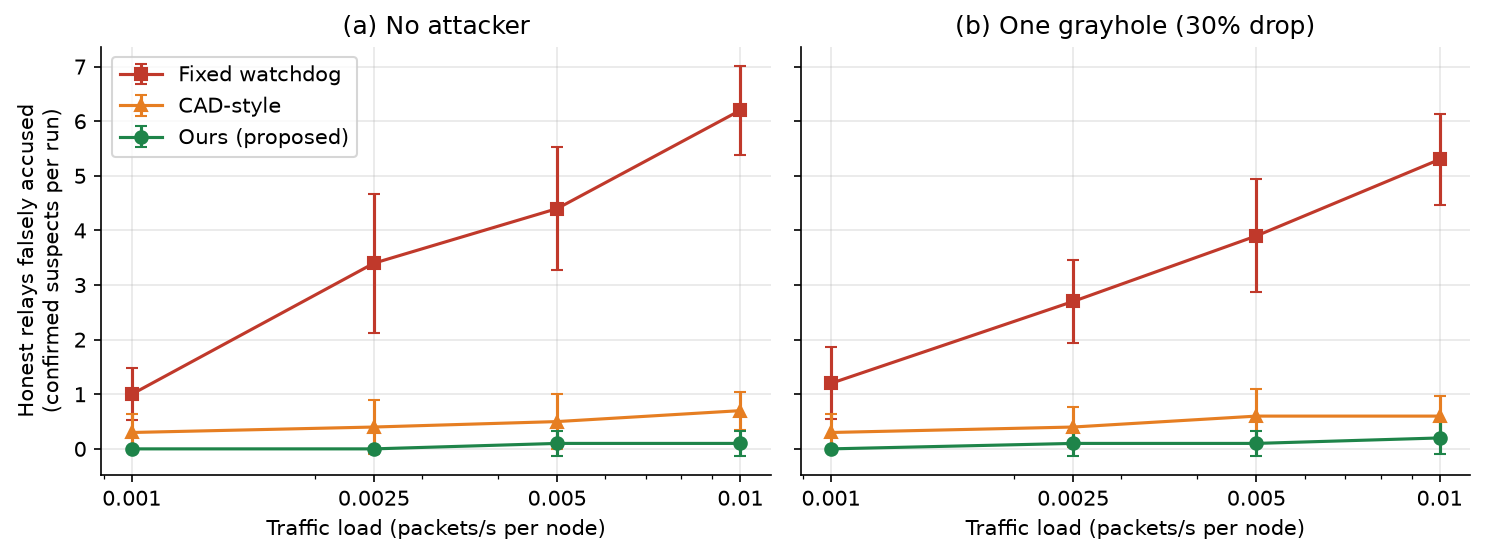
\includegraphics[width=0.9\linewidth]{figs/fig2_false_accusations.png}
\caption{Honest relays falsely accused per run as the traffic load changes, each method with its own rule (6 h recorded runs, ten test topologies, 95\% $t$-intervals). (a) No attacker. (b) One grayhole that drops 30\%.}\label{fig:fig2}
\end{figure}

\subsection{Drop estimate and ranked suspect list}\label{sec:res-list}
\noindent
Figure~\ref{fig:drop} shows that our estimate follows the true drop rate.
For true rates of 10, 20 and 50\%, our estimates are 7.6, 18.8 and 47.2\%.
For the same cases, the CAD-style score gives 0.0, 1.2 and 31.3\%, so it underestimates moderate dropping.
Table~\ref{tab:list} is the list that the administrator receives for test topology 201 with three grayholes after six hours.
The three grayholes are first in the list, and the sink confirms them.
The estimate for each honest relay is 0 to 0.2\%.

\begin{figure}[htbp]
\centering
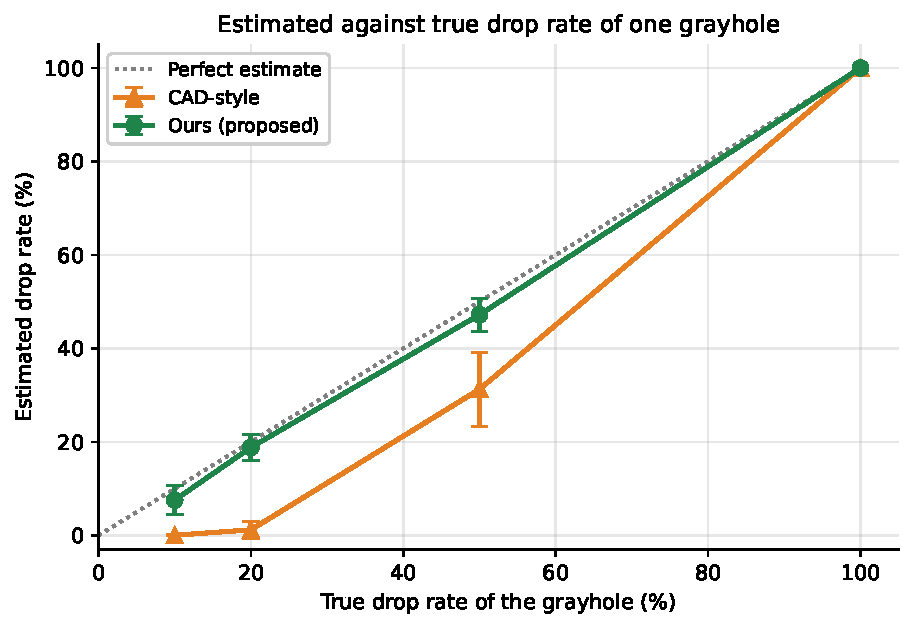
\includegraphics[width=0.55\linewidth]{figs/drop_estimate.pdf}
\caption{Estimated and true drop rate of one grayhole (load 0.005, ten test topologies, 95\% $t$-intervals).}\label{fig:drop}
\end{figure}

\begin{table}[htbp]
\centering\small
\caption{Ranked suspect list from our detector (test topology 201, three grayholes that drop 30\%, load 0.005, after 6 h).}\label{tab:list}
\begin{tabular}{c c c c c c c}
\toprule
Rank & Node & Estimated drop & Trust & Windows & Decision & Truth \\
\midrule
1 & 17 & 38.9\% & 0.61 & 1253 & Suspect & Grayhole \\
2 & 10 & 32.1\% & 0.68 & 3393 & Suspect & Grayhole \\
3 & 12 & 28.2\% & 0.72 & 1733 & Suspect & Grayhole \\
4 & 16 & 0.2\% & 1.00 & 246 & None & Honest \\
5 & 8 & 0.0\% & 1.03 & 415 & None & Honest \\
6 & 4 & 0.0\% & 1.02 & 217 & None & Honest \\
7 & 5 & 0.0\% & 1.08 & 102 & None & Honest \\
\bottomrule
\end{tabular}
\end{table}

\subsection{Effect of the attack and detection time}\label{sec:res-attack}
\noindent
Table~\ref{tab:attack} compares each attack with the same networks without attack (load 0.005, no defence).
One grayhole decreases the delivery ratio by 8.4\%, two by 14.2\% and three by 17.0\%.
Each added grayhole removes less than the one before, because the attack starts at the busiest relay.
Confirmation needs two flagged rounds, so the earliest detection time is 60 minutes.
The mean time for our detector to confirm every grayhole increases from 97 to 140 minutes as we add grayholes.
Several grayholes hide one another until the baseline cleaning removes them.

\begin{table}[htbp]
\centering\small
\caption{Effect of the attack and detection time (live network, 12 h, ten test topologies, load 0.005).}\label{tab:attack}
\begin{tabular}{c c c c c}
\toprule
Grayholes & \shortstack{Delivery,\\no attack} & \shortstack{Delivery,\\attack, no defence} & \shortstack{Decrease\\(absolute)} & \shortstack{Time to confirm\\all grayholes (ours)} \\
\midrule
1 & 60.5\% & 52.1\% & 8.4\% & 97 min \\
2 & 59.6\% & 45.4\% & 14.2\% & 127 min \\
3 & 59.2\% & 42.2\% & 17.0\% & 140 min \\
\bottomrule
\end{tabular}
\end{table}

\subsection{Route-around response}\label{sec:res-route}
\noindent
With the default response, traffic goes around each suspect where another path exists, and no node is cut off.
Table~\ref{tab:live} gives the results.
Our detector caught 95\% of the grayholes and accused 0.3 honest relays per run.
The fixed watchdog accused 7.2.
Our delivery ratio (49.7\%) is the highest, but its gain over the CAD-style detector (0.7\% to 2.7\% per setting) is inside the 95\% interval.
Thus we do not claim a delivery gain for this response.

\begin{table}[htbp]
\centering\small
\caption{Route-around response (live network, 12 h, ten test topologies, four attack settings).}\label{tab:live}
\begin{tabular}{l c c c}
\toprule
Method & \shortstack{Grayholes\\caught} & \shortstack{Honest relays\\accused per run} & \shortstack{Delivery\\ratio} \\
\midrule
No attack & n/a & n/a & 57.0\% \\
Attack, no defence & 0\% & 0 & 45.6\% \\
Fixed watchdog & 100\% & 7.2 & 47.0\% \\
CAD-style & 58\% & 0.8 & 48.0\% \\
\textbf{Ours} & \textbf{95\%} & \textbf{0.3} & \textbf{49.7\%} \\
\bottomrule
\end{tabular}
\end{table}

\subsection{Comparison with existing approaches}\label{sec:res-compare}
\noindent
We measured the fixed watchdog and the CAD-style detector above.
Both are adaptations.
The fixed watchdog has no pathrater, and the CAD-style detector uses only the downstream estimate of CAD.
We did not implement the other reviewed approaches, so Table~\ref{tab:sota} compares them by their output and their cost.

\begin{table}[htbp]
\centering\footnotesize\setlength{\tabcolsep}{4pt}
\caption{Comparison with the reviewed approaches.}\label{tab:sota}
\begin{tabular}{>{\raggedright\arraybackslash}p{2.4cm} >{\raggedright\arraybackslash}p{3.6cm} >{\raggedright\arraybackslash}p{4.2cm} >{\raggedright\arraybackslash}p{4.4cm}}
\toprule
Approach & Output & Extra traffic & Unobservable forward \\
\midrule
UnetStack3~\cite{brc2021} & Alarm, no attacker named & None; one monitor, four nodes & Counts as a miss \\
ARTMM~\cite{han2015} & Trust value per node & Trust recommendations & Lowers trust \\
TAFLRLR~\cite{han2023} & Next-hop choice & HELLO flooding, recommendations & Counts as abnormal \\
ATEM~\cite{liu2024} & Trust value per node & Trust recommendations & Skips a full cycle, else a failure \\
\textbf{Ours} & Ranked suspects with drop estimate & One report frame per node every 30 min & Window excluded \\
\bottomrule
\end{tabular}
\end{table}

\subsection{Contribution of each part and limits}\label{sec:res-ablation}
\noindent
We removed one part of our detector at a time.
We tuned each variant on the tuning networks, so that it accuses at most 5\% of honest relays when there is no attacker.
Without baseline cleaning, three-grayhole detection decreases from 23 of 30 to 17 of 30.
Without the observability filter, detection is almost the same after two-round confirmation.
But honest accusations increase from 1.1 to 1.5\% in the load sweep.
The main effect of the filter is the low count in Figure~\ref{fig:fig2}.
Our detector sends approximately 10\% more report frames than the baselines (857 to 973 against 781 to 886 per run), because every monitor reports on every relay that it overhears.
The limits are static topologies, a known loss curve, truthful monitors and free route updates.

%==========================================================
\section{Conclusions and future work}\label{sec:conclusion}
\noindent
The purpose of this work was to find grayhole relays in underwater acoustic networks without accusing honest relays.
An honest relay can lose forwards because of half-duplex deafness, collisions or long links.
We built a detector in UnetStack that counts a watch window only when the monitor could observe the forward.
It compares the forwards heard with the forwards that each link must show, and confirms a suspect after two flagged rounds.
Reports go to the sink over the acoustic channel, and the sink ranks the suspects.

On ten test networks, our detector caught 95\% of the grayholes and accused 0.3 honest relays per run.
The fixed watchdog accused 7.2.
Its drop estimate was within 3\% of the true rate.
With blacklisting, it kept a delivery ratio of 45.7\%, and the fixed watchdog kept 23.2\%.

Future work must test dishonest monitors, mobile nodes and position errors.
It must also learn the loss curve during operation and decrease false accusations in dense networks.

%==========================================================
\begin{thebibliography}{99}
\small

\bibitem{akyildiz2005}
I. F. Akyildiz, D. Pompili, and T. Melodia, ``Underwater acoustic sensor networks: Research challenges,'' \emph{Ad Hoc Netw.}, vol.~3, no.~3, pp.~257--279, May 2005, doi: 10.1016/j.adhoc.2005.01.004.

\bibitem{karlof2003}
C. Karlof and D. Wagner, ``Secure routing in wireless sensor networks: Attacks and countermeasures,'' \emph{Ad Hoc Netw.}, vol.~1, no.~2--3, pp.~293--315, Sep. 2003, doi: 10.1016/S1570-8705(03)00008-8.

\bibitem{domingo2011}
M. C. Domingo, ``Securing underwater wireless communication networks,'' \emph{IEEE Wireless Commun.}, vol.~18, no.~1, pp.~22--28, Feb. 2011, doi: 10.1109/MWC.2011.5714022.

\bibitem{marti2000}
S. Marti, T. J. Giuli, K. Lai, and M. Baker, ``Mitigating routing misbehavior in mobile ad hoc networks,'' in \emph{Proc. 6th Annu. Int. Conf. Mobile Comput. Netw. (MobiCom)}, Boston, MA, USA, 2000, pp.~255--265, doi: 10.1145/345910.345955.

\bibitem{brc2021}
B. R. Chandavarkar and N. Suresh, ``Demonstration of selective forwarding attack and detection mechanism in UnetStack3,'' in \emph{Proc. 12th Int. Conf. Comput. Commun. Netw. Technol. (ICCCNT)}, Kharagpur, India, 2021, pp.~1--6, doi: 10.1109/ICCCNT51525.2021.9580125.

\bibitem{shila2010}
D. M. Shila, Y. Cheng, and T. Anjali, ``Mitigating selective forwarding attacks with a channel-aware approach in WMNs,'' \emph{IEEE Trans. Wireless Commun.}, vol.~9, no.~5, pp.~1661--1675, May 2010, doi: 10.1109/TWC.2010.05.090700.

\bibitem{han2015}
G. Han, J. Jiang, L. Shu, and M. Guizani, ``An attack-resistant trust model based on multidimensional trust metrics in underwater acoustic sensor network,'' \emph{IEEE Trans. Mobile Comput.}, vol.~14, no.~12, pp.~2447--2459, Dec. 2015, doi: 10.1109/TMC.2015.2402120.

\bibitem{han2023}
D. Han, X. Du, L. Wang, X. Liu, and X. Tian, ``Trust-aware and fuzzy logic-based reliable layering routing protocol for underwater acoustic networks,'' \emph{Sensors}, vol.~23, no.~23, Art.~no.~9323, 2023, doi: 10.3390/s23239323.

\bibitem{liu2024}
C. Liu, J. Ye, F. An, and W. Jiang, ``An adaptive trust evaluation model for detecting abnormal nodes in underwater acoustic sensor networks,'' \emph{Sensors}, vol.~24, no.~9, Art.~no.~2880, 2024, doi: 10.3390/s24092880.

\bibitem{chitre2014}
M. Chitre, R. Bhatnagar, and W.-S. Soh, ``UnetStack: An agent-based software stack and simulator for underwater networks,'' in \emph{Proc. OCEANS 2014}, St. John's, NL, Canada, 2014, pp.~1--10, doi: 10.1109/OCEANS.2014.7003044.

\bibitem{jiang2019}
S. Jiang, ``On securing underwater acoustic networks: A survey,'' \emph{IEEE Commun. Surveys Tuts.}, vol.~21, no.~1, pp.~729--752, 2019, doi: 10.1109/COMST.2018.2864127.

\bibitem{hai2008}
T. H. Hai and E.-N. Huh, ``Detecting selective forwarding attacks in wireless sensor networks using two-hops neighbor knowledge,'' in \emph{Proc. 7th IEEE Int. Symp. Netw. Comput. Appl. (NCA)}, Cambridge, MA, USA, 2008, pp.~325--331, doi: 10.1109/NCA.2008.13.

\bibitem{unethandbook}
UnetStack, ``Unet handbook: Physical service.'' [Online]. Available: \url{https://unetstack.net/handbook/305_phy.html} (accessed Oct. 12, 2026).

\end{thebibliography}

\end{document}
